% interacttfssample.tex
% v1.05 - August 2017

\documentclass[]{interact}

%\usepackage{epstopdf}% To incorporate .eps illustrations using PDFLaTeX, etc.
\usepackage[caption=false]{subfig}% Support for small, `sub' figures and tables
%\usepackage[nolists,tablesfirst]{endfloat}% To `separate' figures and tables from text if required

%\usepackage[doublespacing]{setspace}% To produce a `double spaced' document if required
%\setlength\parindent{24pt}% To increase paragraph indentation when line spacing is doubled
%\setlength\bibindent{2em}% To increase hanging indent in bibliography when line spacing is doubled

\usepackage[numbers,sort&compress]{natbib}% Citation support using natbib.sty
\bibpunct[, ]{[}{]}{,}{n}{,}{,}% Citation support using natbib.sty
\renewcommand\bibfont{\fontsize{10}{12}\selectfont}% Bibliography support using natbib.sty

%\theoremstyle{plain}% Theorem-like structures provided by amsthm.sty
%\newtheorem{theorem}{Theorem}[section]
%\newtheorem{lemma}[theorem]{Lemma}
%\newtheorem{corollary}[theorem]{Corollary}
%\newtheorem{proposition}[theorem]{Proposition}

%\theoremstyle{definition}
%\newtheorem{definition}[theorem]{Definition}
%\newtheorem{example}[theorem]{Example}

%\theoremstyle{remark}
%\newtheorem{remark}{Remark}
%\newtheorem{notation}{Notation}

\begin{document}

{\Large\bf Progress this week}

{\large\bf December 15, 2019}

\begin{itemize}

\item Updated notation.

\item Fit model with covariates.

\end{itemize}

\vfill

\textbf{Previous word count:} 2314 \hfill \textbf{Current word count:} 2342

\textbf{Previous page count:} 9.5 \hfill \textbf{Current page count:} 9.5

\pagebreak

\articletype{REVIEW ARTICLE}% Specify the article type or omit as appropriate

\title{The Integrated Nested Laplace Approximation applied to Spatial Point Process Models}

\author{
\name{Kenneth Flagg\thanks{CONTACT Kenneth Flagg. Email: kenneth.flagg@montana.edu} and Andrew Hoegh}
\affil{Montana State University, Bozeman, MT}
}

\maketitle

\begin{abstract}
This template is for authors who are preparing a manuscript for a Taylor \& Francis journal using the \LaTeX\ document preparation system and the \texttt{interact} class file, which is available via selected journals' home pages on the Taylor \& Francis website.
\end{abstract}

\begin{keywords}
INLA, spatial prediction, log-Gaussian Cox process, spatial point process
\end{keywords}


\section{Introduction}
%  {\bf Introduction:} Please introduce one or more current statistical research methods that have been widely used by other discipline(s) in the Introduction section or divide the discussion into two or more subsections within this Introduction section.

% More introduction, define point process terms.

Spatial prediction is a high-dimensional inference problem. When the goal of
statistical modeling is to produce a graphical map of a random variable over
space, the model ultimately must be able to predict that random variable at
every pixel of the image. A map image will typically be at least several
hundred by several hundred pixels, so in total there can easily be hundreds of
thousands of pixels requiring predictions. Thus, even when a model has only
half a dozen parameters, it may include hundreds of thousands of latent
variables.

Spatial point process models further complicate the situation with difficult
likelihoods. {\it (Cite some computational papers --- Baddely?)} Both maximum
likelihood and Bayesian model fitting require integrating the intensity
function over space, but the integral is generally not available in closed
form. Many methods have been introduced including quadrature-based
approximations {\it (cite Baddeley)}, pseudodata approaches
{\it (cite Baddeley/Berman/Turner etc)}, and Markov chain Monte
Carlo~\cite{moellerwaagepetersen}.

Development of the integrated nested Laplace approximation (INLA) has made
accurate approximate model fitting considerably more feasible for a particular
class of log-Gaussian Cox process (LGCP) models. INLA was developed to fit
Bayesian hierarchical models with many latent Gaussian
variables~\cite{rueetal}. A key part of INLA's computational simplicity is that
it calculates the posterior distribution of each latent Gaussian variable one
at a time; that is, it provides only the posterior marginal distributions
rather than the full joint distribution.

When using a LGCP for spatial mapping, two aspects make INLA a suitable
approach. First, the LGCP is driven by a spatial Gaussian process (GP), so the
latent variables are Gaussian. Second, even though the latent variables are
expected to exhibit spatial dependence, their full joint distribution is not
needed. In most situations it suffices to map their predicted values, variance,
and upper and lower interval bounds pointwise across space.

We focus on spatial mapping using a hierarchical construction of the LGCP, and
do so without discussing many classic spatial point process concepts such as
Gibbs processes, Markov processes, point process densities, or the Papangelou
conditional intensity function. For readers interested in the general spatial
point process context in which the LGCP originates, we recommend other
references~\cite{moellerwaagepetersen, digglepoint, cressie}.

Much recent work in point process modeling involves spatiotemporal models,
which are easily implemented in INLA by allowing the parameters of a spatial
point process model to vary over time. To keep the focus on the spatial
aspects, we do not discuss spatiotemporal models. This article provides a
review of recent advances in the fitting of spatial LGCP models via INLA,
including dimension reduction by triangulation, a likelihood factorization that
avoids gridding, and incorporation of sampling or false negatives.


\subsection{Log-Gaussian Cox Process}

Notes from \cite{moellerwaagepetersen}:

\begin{itemize}

\item applications mentioned: seismology, ecology, forestry, geography, spatial
epidemiology and materials science

\item modern computing (e.g. McMC) allows for model-based inference without a
stationarity assumption

\item Minke whale distance sampling data used as an example of incomplete
observation (they used a shot noise Cox process model)

\item distribution of point process is the joint distrubition of \(n\) and
the \(n\) events, or equivalently the distribution of the number of events in
any arbitrary region

\item in their presentation of the two Poisson process postulates, the second
one is given the number of events in a region they are iid proportional to the
intensity function

\item Cox process is driven by a non-negative random process such that
conditional on the driving process the Cox process is a Poisson process

\item LGCP has no edge effects because the point process in the window is
fully specified by the GP restricted to the window

\item quite a bit about Gibbs processes, densities wrt stationary Poisson
processes, and Papangelou conditional intensities (comments: The density was
traditionally used to facilitate McMC simulation and ML fitting when the
likelihood was not explicitly available. The conditional intensity of a
Poisson process is the intensity function because of independence among the
points. The hierarchical setup of the LGCP lets us work directly with a
Poisson process so the density and conditional intensity are not needed. LGCP
models with constructed covariate can model Gibbs processes.)

\item more things about infinite Gibbs and Markov processes that go over my
head but we don't need because we deal with bounded and finite processes

\end{itemize}

Notation and terminology:

\begin{itemize}

\item process defined on \(\mathcal{D} \subset \mathbb{R}^{2}\), domain of the
intensity function, define \(d = \mathrm{dim}(\mathcal{D})\)

\item observation window \(\mathcal{S} \subset \mathcal{D}\)

\item \emph{(Note: When thinking about sampling, we need to define three
regions: the domain \(\mathcal{D}\) over which the process mathematically
operates, the region \(\mathcal{R}\) over which inferences are desired, and
the observed/sampled observation window \(\mathcal{S}\). The general
relationship is \(\mathcal{S} \subset \mathcal{R} \subset \mathcal{D}
\subset \mathbb{R}^{d}\), where all of the subset symbols taken to mean
``subset or equal''. The ``fully surveyed'' situation is \(\mathcal{S}
= \mathcal{R}\).)}

\item \(\mathbf{X}\) point process on \(\mathcal{R}\),
\(\mathbf{x} = \{x_{1}, \dots, x_{n}\}\) realized point pattern

\item point \(x \in \mathbf{x}\) called an event

\item intensity function \(\lambda(u)\)

\item \(x\) event, \(s\) numerical integration node, \(u\)
arbitrary location in \(\mathcal{D}\)

\item \(z(u)\) a column vector of covariates/predictors at \(u\)

\item ``point'' refers to a \(u\) unless clearly stated otherwise

\item bold for sets and spatial processes, normal italics for spatial vectors

\item \(y\) and variations will be used for objects derived from the point
pattern, e.g. pseudodata

\end{itemize}


The LGCP is a Poisson process driven by a latent Gaussian
process~\cite{moelleretal}. A Poisson process is characterized entirely by its
intensity function \(\lambda(u)\), which gives the mean number of events
per unit area, and the process satisfies the following two properties
{\it (find a good citation)}.
\begin{enumerate}
\item The number of events in any region \(\mathcal{B}\) follows a Poisson
distribution with mean
\(\int_{\mathcal{B}} \lambda(u)\mathrm{d}u\).
\item The numbers of events in disjoint regions are independent.
\end{enumerate}

Commonly, covariates are incorporated via a log-linear model for the intensity,
\begin{displaymath}
\log\lambda(u) = \mathbf{z}'(u) \boldsymbol{\beta}.
\end{displaymath}
The LGCP adds another stochastic layer,
\begin{displaymath}
\log\lambda(u) = \mathbf{z}(u)' \boldsymbol{\beta} + \boldsymbol{\Psi}(u),
\end{displaymath}
where \(\boldsymbol{\Psi}\) is a Gaussian process.

Where the spatial Poisson process has a (stochastically) fixed intensity to be
estimated from data, the spatial LGCP induces a hierarchical model where the
intensity function is itself a random process to be predicted.

% Need to better explain the hierarchical setup. Separate Poisson process from
% GP and write out likelihoods separately?

M\"{o}ller and Waagepetersen (2007) present model checking tools for LGCP
models~\cite{moellerwaagepetersen}.


\subsection{Integrated Nested Laplace Approximation}

INLA was developed with the goal of providing fast, accurate, deterministic
approximations for posterior marginal distributions of the parameters in
latent Gaussian models~\cite{rueetal}. The setting is Bayesian generalized
additive models but is kept very general; this includes linear models, models
with nonlinear (spline, random walk, etc.) functions of predictors, and models
with temporal and/or spatial dependence. Such models commonly have a large
number of Gaussian latent variables or parameters with Gaussian priors and
relatively few non-Gaussian parameters. The INLA approach makes repeated use
of Laplace expansion, numerical integration, and numerical search. The method
has established usefulness for LGCP~\cite{illianetal}. It is readily
implemented using the standalone INLA software or in R via the
R-INLA package~\cite{inlar}.

% Define some coherent notation, then come back and spell out the algorithm.

%- $\mathbf{y} = (y_{1}, \dots, y_{n})'$ independent Gaussian observations

%- $y_{i} \sim \mathrm{N}(\theta, \sigma^{2})$

%- $\theta \sim \mathrm{N}(\mu_{0}, \sigma_{0}^{2})$

%- $\psi = 1/\sigma^{2}$, $\psi \sim \mathrm{Gamma}(a, b)$

%- The posterior distribution of $\psi$:
%$$p(\psi|\mathbf{y}) \propto \frac{p(\mathbf{y} | \theta, \psi) p(\theta) p(\psi)}
%{p(\theta | \psi, \mathbf{y})}$$

%- Laplace approximation:
%$$\tilde{p}(\psi|\mathbf{y}) \propto \frac{p(\mathbf{y} | \theta, \psi) p(\theta) p(\psi)}
%{\tilde{p}_{G}(\theta^{*} | \psi, \mathbf{y})}$$

%Repeat for $\theta$, will depend on $\psi$

%Provides marginal posteror for one entry at a time of a vector $\boldsymbol{\theta}$


\section{Methodology}
%  {\bf Methodology or Approach:} Present the method(s) and relevant applications being reviewed in this or more sections.

INLA provides an efficient computational framework for fitting Bayesian models
with latent Gaussian variables. On top of this framework are built several
tools to further simplify the fitting of spatial LGCP models. The stochastic
partial differential equation (SPDE) approach provides dimension reduction for
the spatial GP~\cite{lindgrenetal}. The SPDE approach employs a numerical
integration scheme which can also be used to approximate the LGCP likelihood
and negate the need to grid the events into Poisson counts~\cite{simpsonetal}.
With these computational improvements, researchers are now able to efficiently
fit LGCP models to incompletely-observed point patterns~\cite{yuanetal}.  


\subsection{The SPDE Approach}

Because the LGCP includes a Gaussian process (GP), efficient computation for
Gaussian processes is critical when working with LGCP models.

The GP imposes a dense covariance matrix on the latent variables~\cite{rinla}.
For GPs with a Mat\'{e}rn covariance function, a Gaussian Markov random field
(GMRF) approximation can simplify computation, requiring only a sparse
covariance structure.

The GMRF approximation is motivated by the fact that Gaussian fields with
Mat\'{e}rn covariances are solutions to the below stochastic partial
differential equation (SPDE)~\cite{lindgrenetal}.
\begin{displaymath}
(\kappa^{2} - \Delta)^{\alpha / 2} \boldsymbol{\Psi}(u) = \mathbf{W}(u),
\qquad u \in \mathbb{R}^d, \quad \kappa > 0,
\quad \alpha = \nu + d/2, \quad \nu > 0
\end{displaymath}
Here, \(\mathbf{W}\) is a Gaussian white noise process with variance 1, and
\(\Delta\) is the Laplacian operator. The stationary solution
\(\boldsymbol{\Psi}\) is a Gaussian field with a Mat\'{e}rn covariance function
with scaling parameter \(\kappa\) (approximately inversly proportional to the
range) and smoothness parameter \(\nu\). The variance is a function of
\(\kappa\), \(\nu\), and \(d\).

Lindgren, Rue, and Lindstr\"{o}m investigate the limit as \(\nu \to 0\) for
\(d = 2\), finding that the solution is a GMRF on a unit
lattice~\cite{lindgrenetal}. They then construct approximations for positive
integer values of \(\nu\) by \(\nu\)-fold convolution of \(\boldsymbol{\Psi}\)
with itself. Finally, they use a finite element method to genrealize the
approximation to arbitrary triangulations of the support. This approximation
has considerable computational benefits because the GMRF has a sparse
covariance structure; the only nodes with nonzero covariances are those
 directly connected by edges in the triangulation.

In practice, the SPDE approach goes as follows. Choose nodes \(s_{i}\)
at which to model \(\boldsymbol{\Psi}(s_{i})\), then build a triangular mesh
using these nodes. Typically the nodes will include locations where data or
covariates are available, then the rest will be filled in with a Delaunay
triangulation under some edge length constraints. The
\(\boldsymbol{\Psi}(s_{i})\) are modeled as a GMRF where the distribution of
each \(\boldsymbol{\Psi}(s_{i})\) depends only on the
\(\boldsymbol{\Psi}(s_{j})\) where \(s_{i}\) and \(s_{j}\) are connected by an
edge. The GMRF representation is assumed to be a piecwise linear approximation
of the continuous Gaussian field; values of \(\boldsymbol{\Psi}(s)\) for
\(s\) not in the set of nodes are predicted by linear interpolation using
the barycentric coordinates of \(s\).

% Add some of the linear algebraic notation and basis function discussion.

% Add comments about coursenes/fineness of mesh.

%Computationally doable when \(Z(\mathbf{s})\) has a Mat\'{e}rn covariance with
%certain values of the smoothness parameter. Check newer references.

\begin{figure}[p]
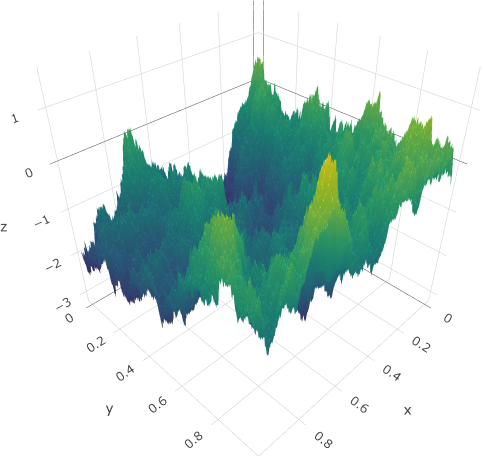
\includegraphics[width=\textwidth]{figures/surface.png}
\caption{A realization of a spatial Gaussian process (left) and an
approximation of that realization over a triangular mesh (right).}
\label{surface}
\end{figure}

\begin{figure}[p]
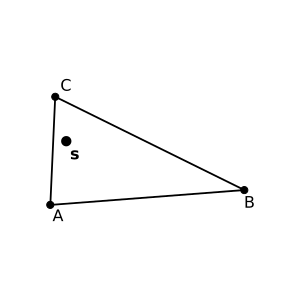
\includegraphics[width=0.5\textwidth]{figures/triangle.png}
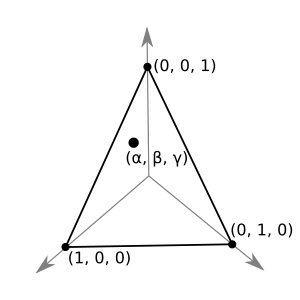
\includegraphics[width=0.5\textwidth]{figures/simplex.png}
\caption{An illustration of the linear transformation from a mesh triangle to
the simplex. \((\alpha, \beta, \gamma)\) are the barycentric coordinates of
\(u\).}
\label{triangle}
\end{figure}

\begin{figure}[h]\centering
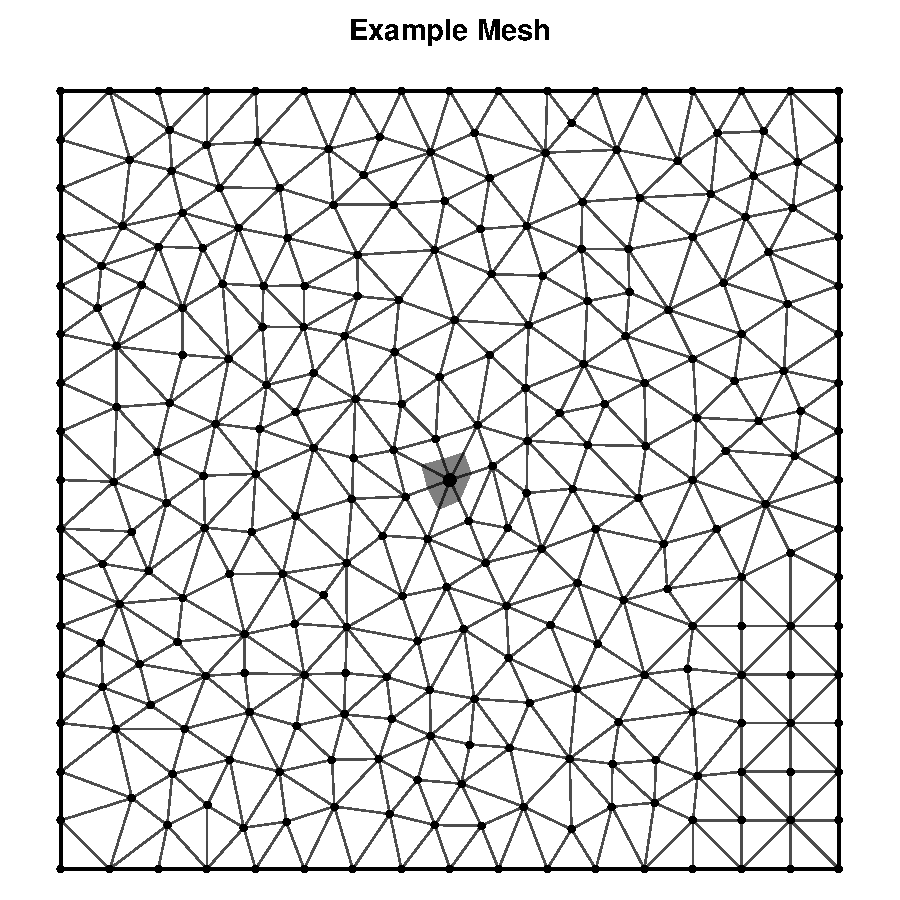
\includegraphics[width=0.5\textwidth]{figures/dual.pdf}
\caption{An illustration of the nodes (dots) and the weighting scheme for one
node (large dot). This node represents the shaded region, so its weight is
proportional to the shaded area. The shaded region is constructed by connecting
the midpoints of the node's edges.}
\label{dual}
\end{figure}

The SPDE approach is implemented in the \texttt{R-INLA} package along with
tools for constructing meshes. A wrapper for easily fitting LGCP models is
provided in the \texttt{inlabru} package~\cite{inlabru}.


\subsection{Going Off the Grid}

Point pattern data are sometimes known as presence-only data, underscoring
the fact that information about where events did \emph{not} occur is both
important and often overlooked. There have been many proposed methods to
account for regions that were observed to contain no events (in contrast to
unobserved regions where it is unknown if any events are present). Many of
these methods involve imputation of dummy points or discretization. In the
world of maximum likelihood, perhaps the most well-developed of these use
approximations based on logistic regression on presence/absence information in
small disjoint regions {\it (cite a bunch of Baddely etc papers)}.
% What is the state-of-the-art for dummy point selection? The papers I'm
% familiar with use lattices or SRSs. Space-filling approaches?

Another alternative, which is probably the most popular approach to Bayesian
fitting of LGCP models but is also common in frequentist analyses, is to grid
the domain and model the induced Poisson counts. It has long been understood
that results are sensitive to the discretization scheme~\cite{brixmoeller}.
Simpson et. al. (2016) explain that this is also computationally
wasteful~\cite{simpsonetal}.
% Tradeoff: small grid cells for spatial precision vs small number of zeros
% for computational speed.

Simpson et. al. took LGCP inference ``off grid'' by intoducing a
computationally-efficient approximation to the Poisson process likelihood that
requires the intensity function only to be evaluated at the locations of
observed events and at the nodes of a mesh. Thus, the SPDE approach can be
employed to model the intensity surface and the same nodes reused in
evaluation of the Poisson process likelihood. The result is a substantial
improvement in both computing time and accuracy of the approximation compared
to gridding.

% Thought on efficiency: fine grid is needed for precision regarding event
% locations? Are there efficient adaptive grid methods?

The approximation arises from a factorization of the Poisson processes
likelihood. The exact log-likelihood is
\begin{displaymath}
\ell(\lambda) = C - \int \lambda(u) \mathrm{d}u
+ \sum_{i = 1}^{n} \log\left[\lambda(x_{i})\right]
\end{displaymath}
where \(C\) is a normalizing constant. The log-intensity is projected into the
space spanned by a finite set of basis function
representation is used for \(\log[\lambda(u)]\), namely
\begin{displaymath}
\log\left[\lambda(u)\right]
\approx \sum_{j = 1}^{m} \psi_{j} \phi_{j}(u)
\end{displaymath}
with \(\boldsymbol{\psi} = (\psi_{1}, \dots, \psi_{m})'\) a multivariate
normal random vector and \(\{\phi_{1}, \dots, \phi_{m}\}\) a set of linearly
independant basis functions.
% The basis function representation is actually the SPDE representation.
% Say so and move this to the previous section.
This defines a numerical integration scheme at nodes \(s_{i}\)
with weights \(\alpha_{i}\) and yields the approximation,
\begin{align*}
\ell(\lambda) &\approx C - \sum_{i = 1}^{m} \tilde{\alpha}_{i}
\exp\left[\sum_{j = 1}^{m} \psi_{j}\phi_{j}(s_{i})\right]
+ \sum_{i = 1}^{n} \sum_{j = 1}^{m} \psi_{j}\phi_{j}(x_{i}) \\
& = C - \boldsymbol{\alpha}'
\exp\left[\mathbf{A}_{1} \boldsymbol{\psi}\right]
+ \mathbf{1}' \mathbf{A}_{2} \boldsymbol{\psi}.
\end{align*}
This is equivalent to the likelihood of independent Poisson random variables
with means {\it (translate the confusing algebra from the appendix)}. Thus,
the SPDE approach, which can be easily fit in R-INLA, can be combined with a
Poisson GLM to rapidly fit a LGCP model. There is no need to compute grid
counts, only to define dummy points at the mesh nodes.

% Include a figure showing a dual mesh and explain the alphas.


\subsection{Variable Sampling Effort}

There has long been a gap between point process modeling theory and practice,
where point process models are only fit to data from completely-observed
domains under the assumption that every event was detected perfectly. In
practice, this is not the case as it may be impossible or impractical to census
the entire region of interest. For example, line-transect surveys routinely
generate point pattern data but are analyzed after aggregation rather than
using a point process model. Another issue is that of false negatives, in other
words events which exist but are not detected during the survey. False
negatives are an accepted part of species abundance surveys, where the species
of interest may be camouflaged or hidden in thick plant cover.

The idea of the incompletely-observed domain has been around for some time.
Brix and M\"{o}ller (2001) fit an LGCP model to weed data observed in
rectangular frames and used a Metropolis-adjusted Langevin algorthim
to predict the intensity outside of the observed frames~\cite{brixmoeller}.
Chakraborty et. al (2011) discuss nonhomogeneous Poisson process modeling as
a richer alternative to ecological presence/absence models and describe their
data as ``degraded'' in the sense that sampling bias prevented the entire
region from being fully observed; they fit their model by aggregating the
point pattern to counts in grid cells and using MCMC~\cite{chakrabortyetal}.

With INLA, the SPDE approach, and the ``off grid'' approximation
facilitating the routine fitting of LGCP models, there is now renewed interest
in accounting for variable sampling effort in spatial point process
models~\cite{simpsonetal,yuanetal}.

Sampling effort is accounted for using the theory of thinned point processes.
Thinning refers to the events of one point process being kept or discarded
probabilistically. Let \(\lambda(u)\) be the intensity of the parent process,
and let an event at \(u\) (if it exists) be observed with probability
\(p(u)\). The observed point process is a thinned point process with
intensity
\begin{displaymath}
\lambda_{p}(u) = p(u) \lambda(u),
\end{displaymath}
and if the parent process is a Poisson process then the observed process is
also a Poisson process~\cite{moellerwaagepetersen}.

We seek to make posterior inferences about the parent intensity,
\(\lambda(u)\). If \(p(u)\) is known, its value at each node is used to
adjust the SPDE integration weights. Most usefully, if it is known that
\(p(s) = 0\) at certain nodes \(s\) because they were outside the sruveyed
domain, the weights become zero so those nodes do not contribute to the
integral. If \(p(u)\) is unknown, it can be modeled. Taking the logarithm of
the above and substituting in the basis function representation, we have the
log-linear model
\begin{displaymath}
\log\left[\lambda_{p}(u)\right]
= \log\left[p(u)\right] + \sum_{j = 1}^{m} \psi_{j} \phi_{j}(u).
\end{displaymath}
Thus, any log-linear model for \(p(u)\) that can be fit by INLA and the SPDE
approach can be incorporated into the LGCP model. For example, Yuan et. al
(2017) fit such a model to data from a line-transect survey using a spline
model to account for the unknown detection function~\cite{yuanetal}.


\section{Applications}
%  {\bf Application of your Methodology:} Present some applications of the reviewed methods to some recent data in this or more sections. Also note: Simulation studies can be presented as a sub-section in this section or in a new standalone section.


\subsection{Simulation Study}

ideas:

simulate LGCPs

fit via Simpson method

vary mesh coarseness

explore complexity of predictors vs latent GP

explore bias/variability in parameter posteriors

explore spatial prediction error in latent GP


\subsection{Data Application}

{\it Examples with data, maybe \texttt{bei} dataset or Victorville. Should read
like a tutorial because there aren't many good resources yet.}

\subsubsection{Data and Model}

For an example analysis of real-world data, we consider the locations of
3605 \emph{Beilschmiedia pendula Lauraceae} trees in a tropical
rainforest~\cite{moellerwaagepetersen}. The data are available as the
\texttt{bei} dataset in the \texttt{spatstat} R package~\cite{spatstat}.
The point pattern exhibits inhomogeneity~(Figure~\ref{bei}) which appears
to be associated with elevation~(Figure~\ref{beielev}) and the magnitude of
the gradient~(Figure~\ref{beigrad}).

\begin{figure}[h]
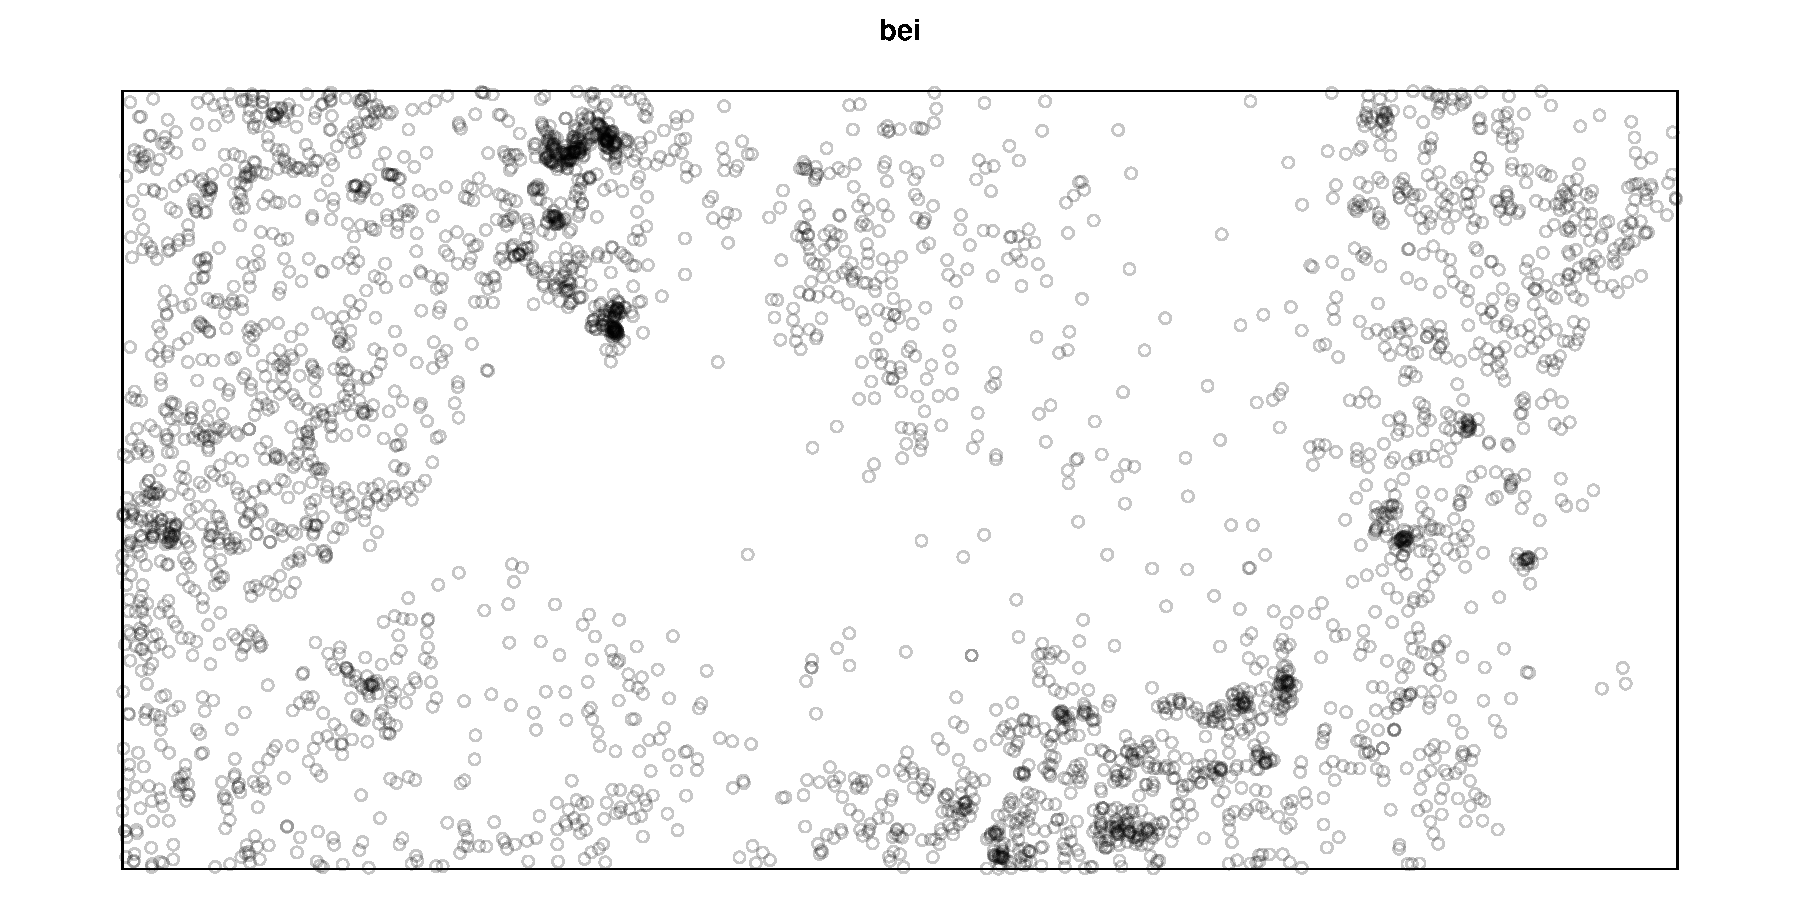
\includegraphics[width=\textwidth]{figures/bei.pdf}
\caption{Locations of trees (events).}
\label{bei}
\end{figure}

\begin{figure}[h]
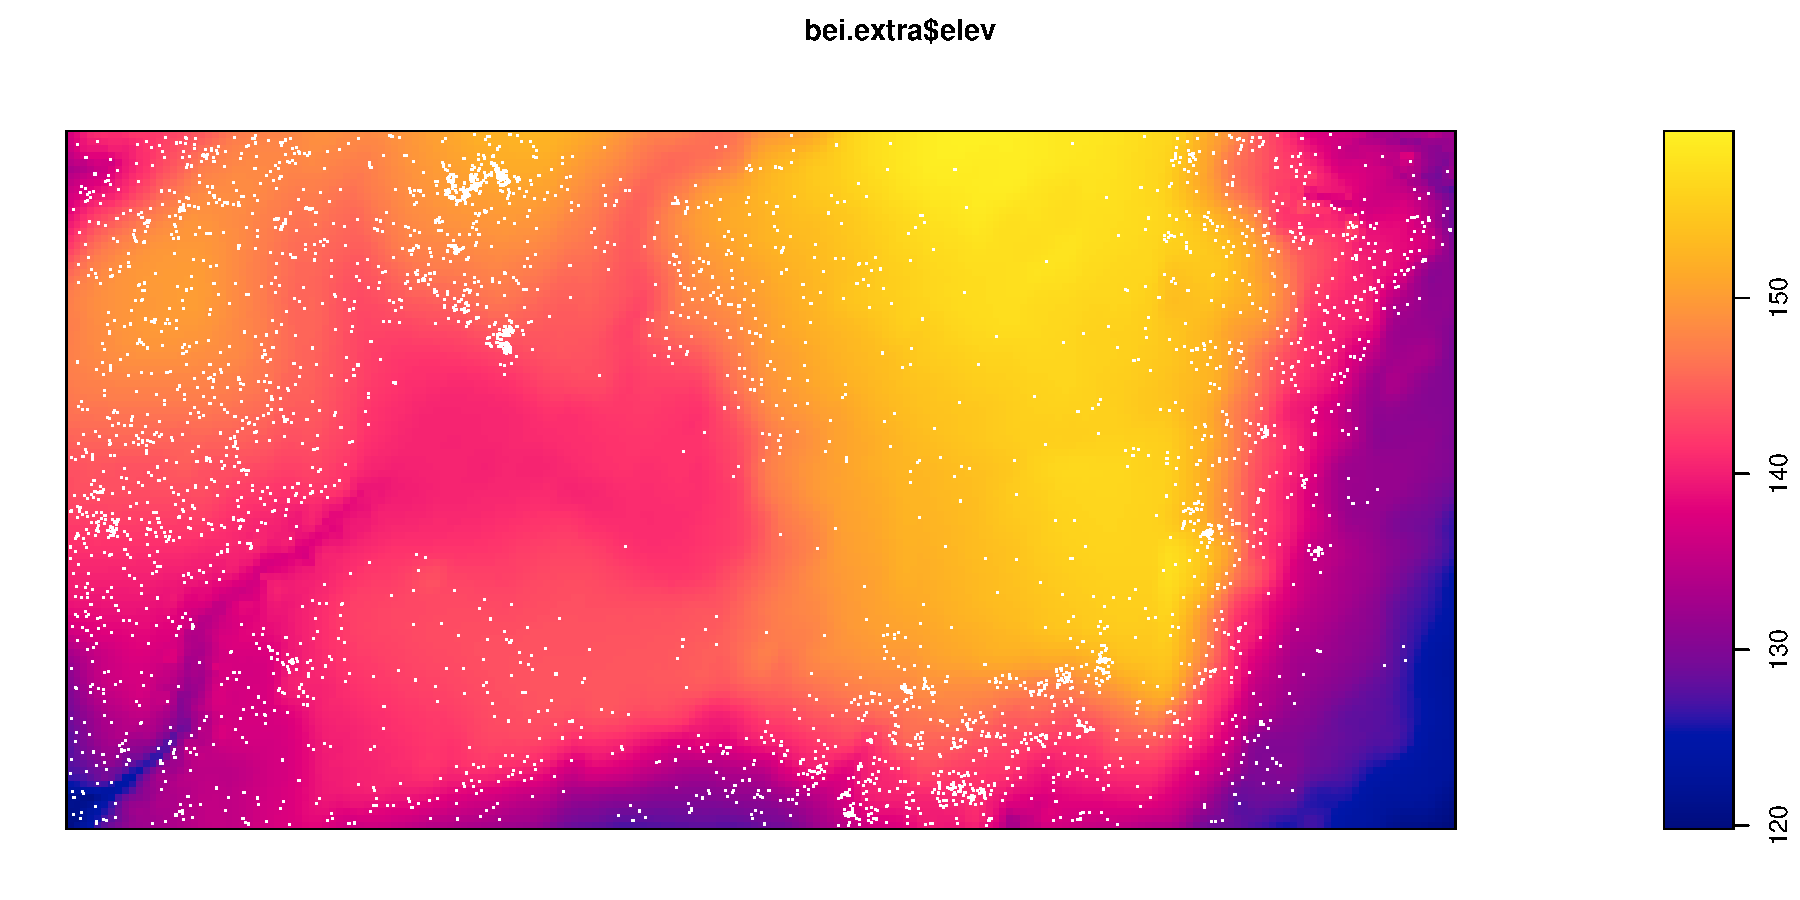
\includegraphics[width=\textwidth]{figures/beielev.pdf}
\caption{Elevation data.}
\label{beielev}
\end{figure}

\begin{figure}[h]
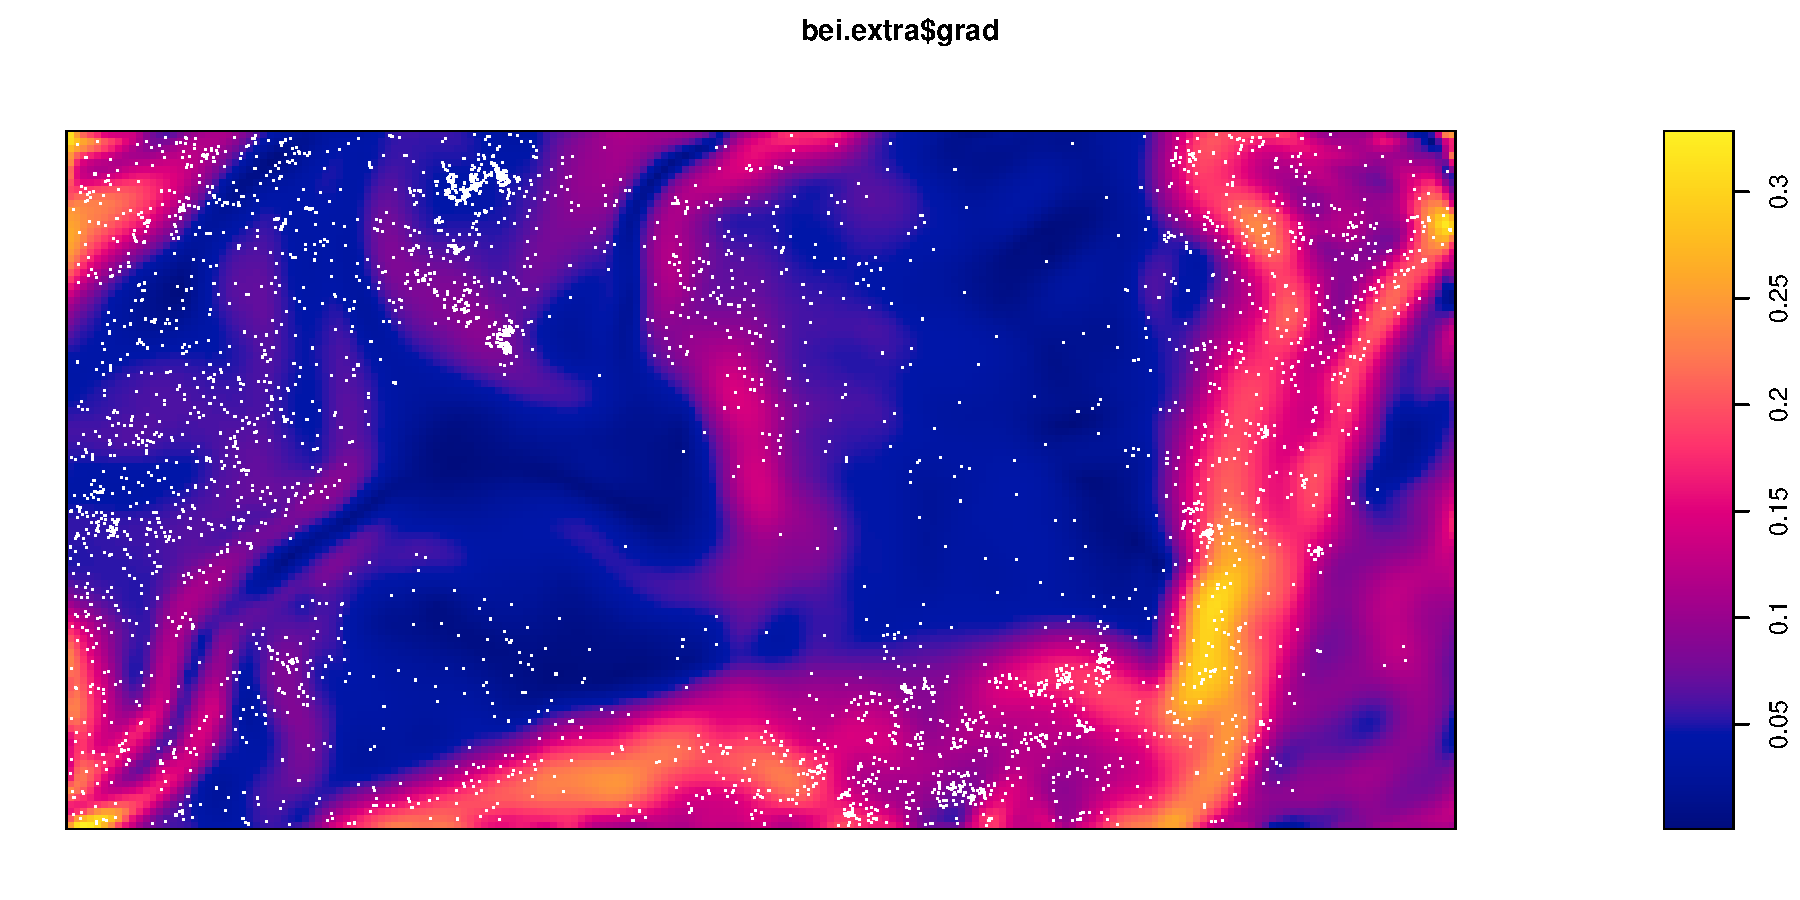
\includegraphics[width=\textwidth]{figures/beigrad.pdf}
\caption{Gradient data.}
\label{beigrad}
\end{figure}


\subsubsection{Fitting in R-INLA}

explain the mesh

\begin{figure}[h]
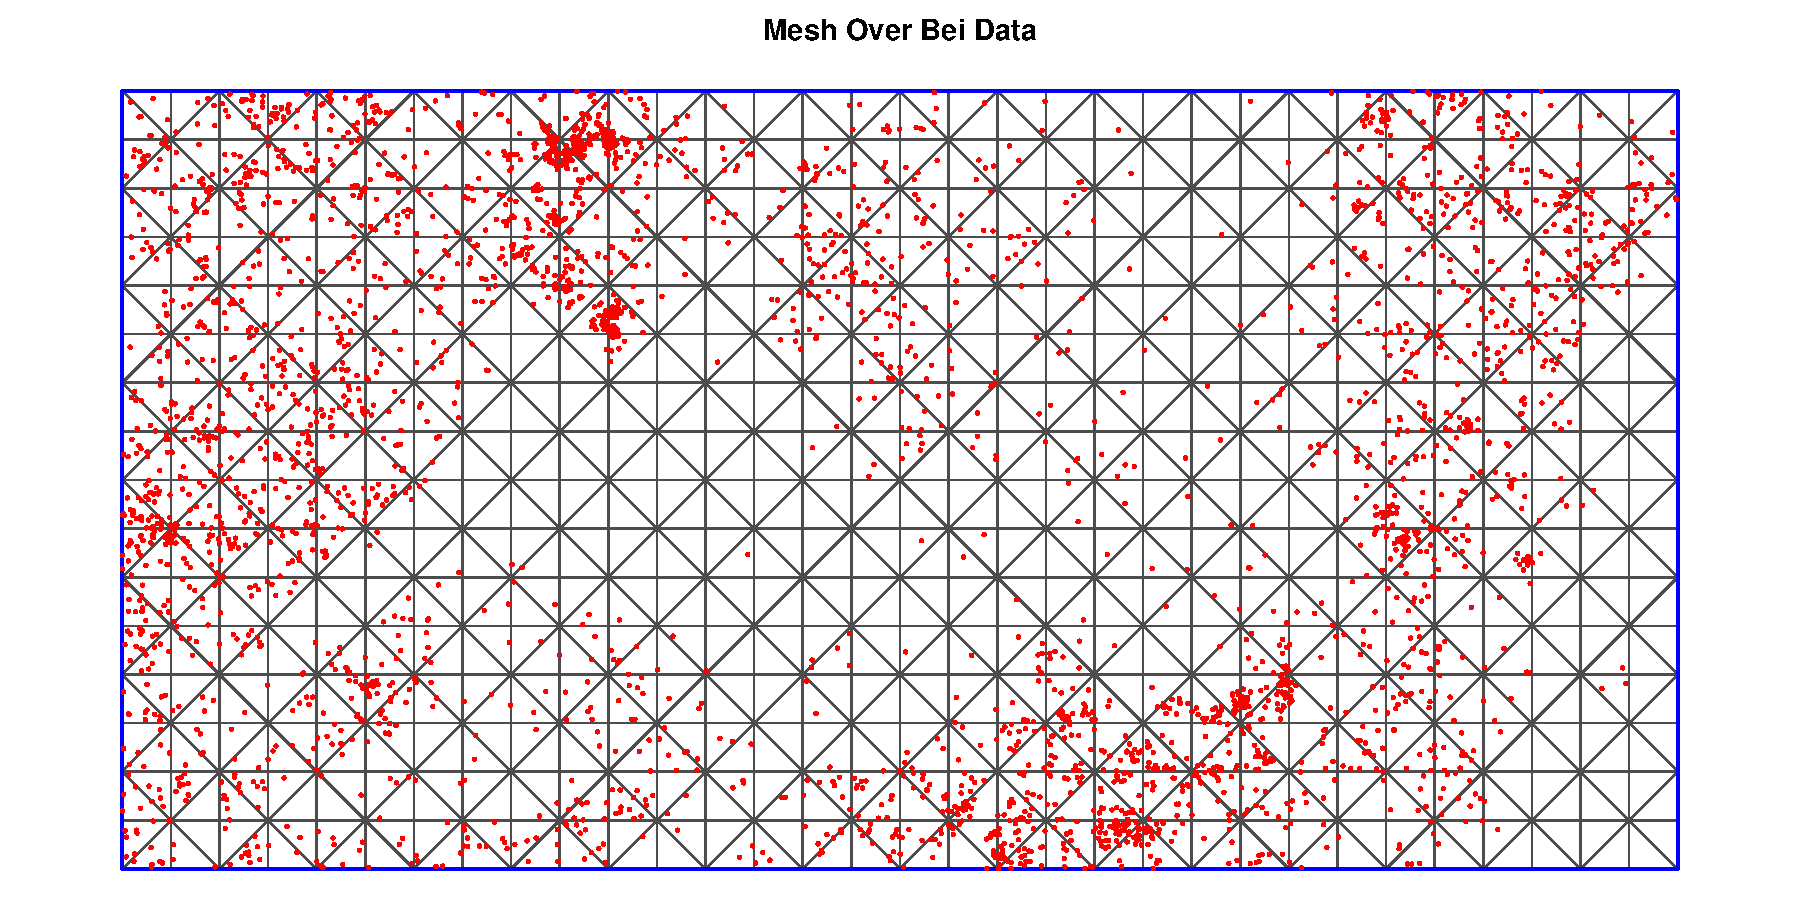
\includegraphics[width=\textwidth]{figures/beimesh.pdf}
\caption{Triangular mesh with events overlaid.}
\label{beimesh}
\end{figure}

explain the weight calculations

walk through the spatial predictions

\begin{figure}[h]
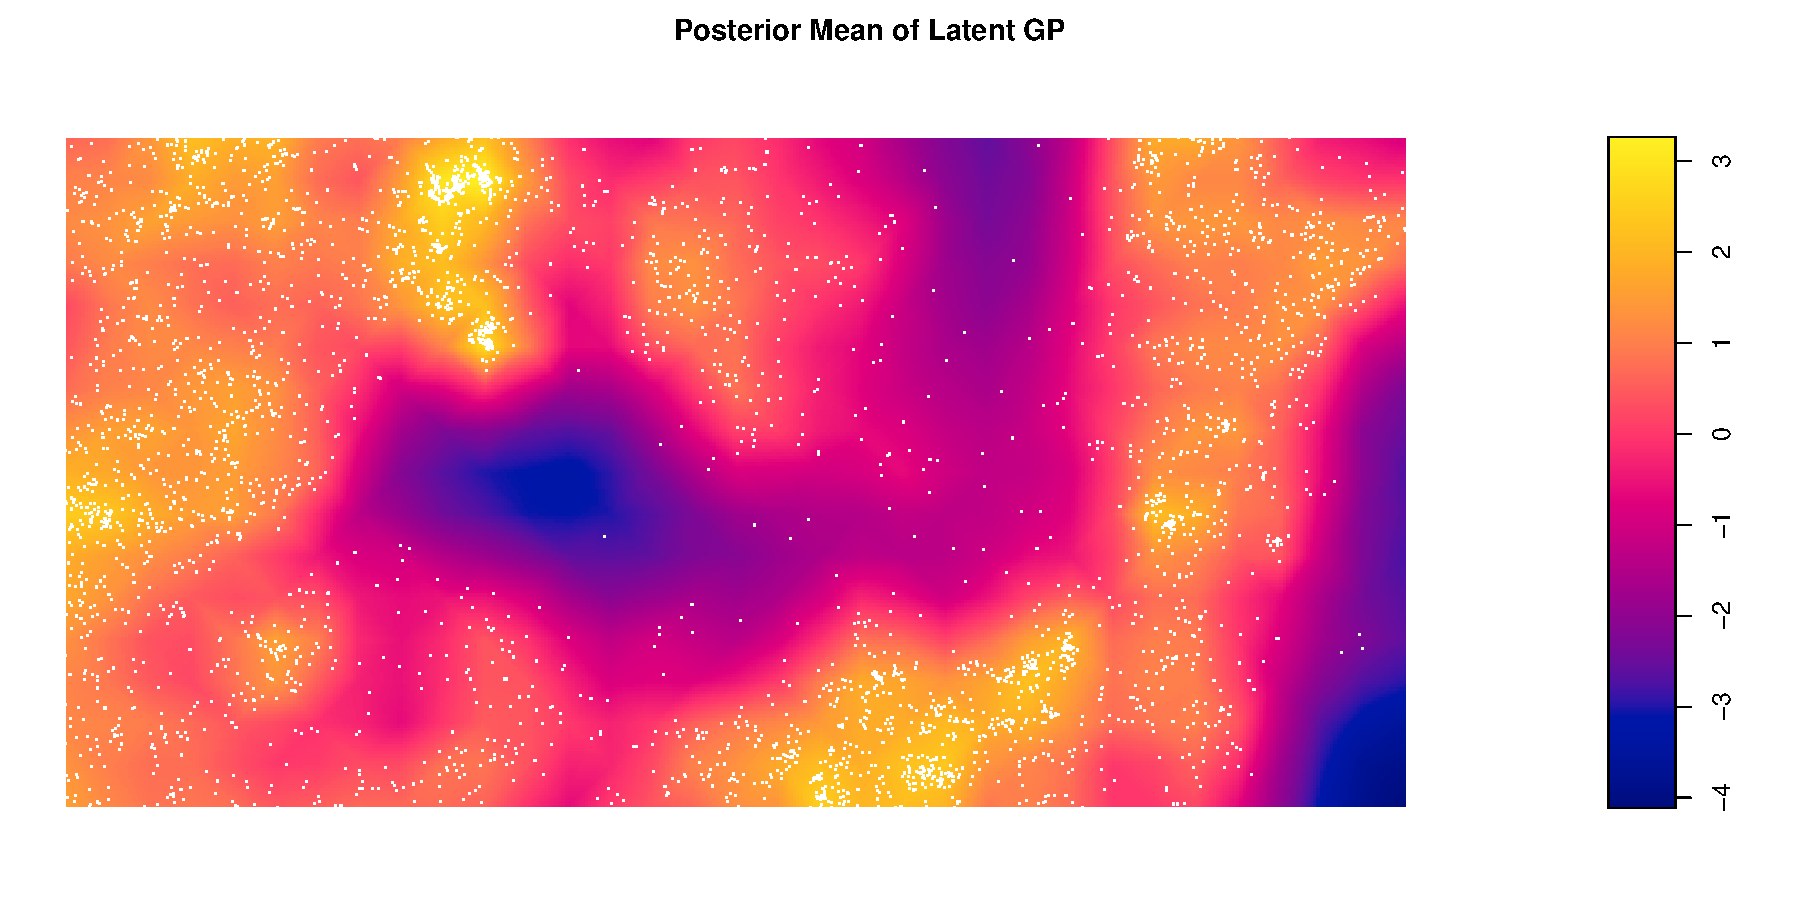
\includegraphics[width=\textwidth]{figures/beimean.pdf}
\caption{Posterior mean prediction surface.}
\label{beimean}
\end{figure}

\begin{figure}[h]
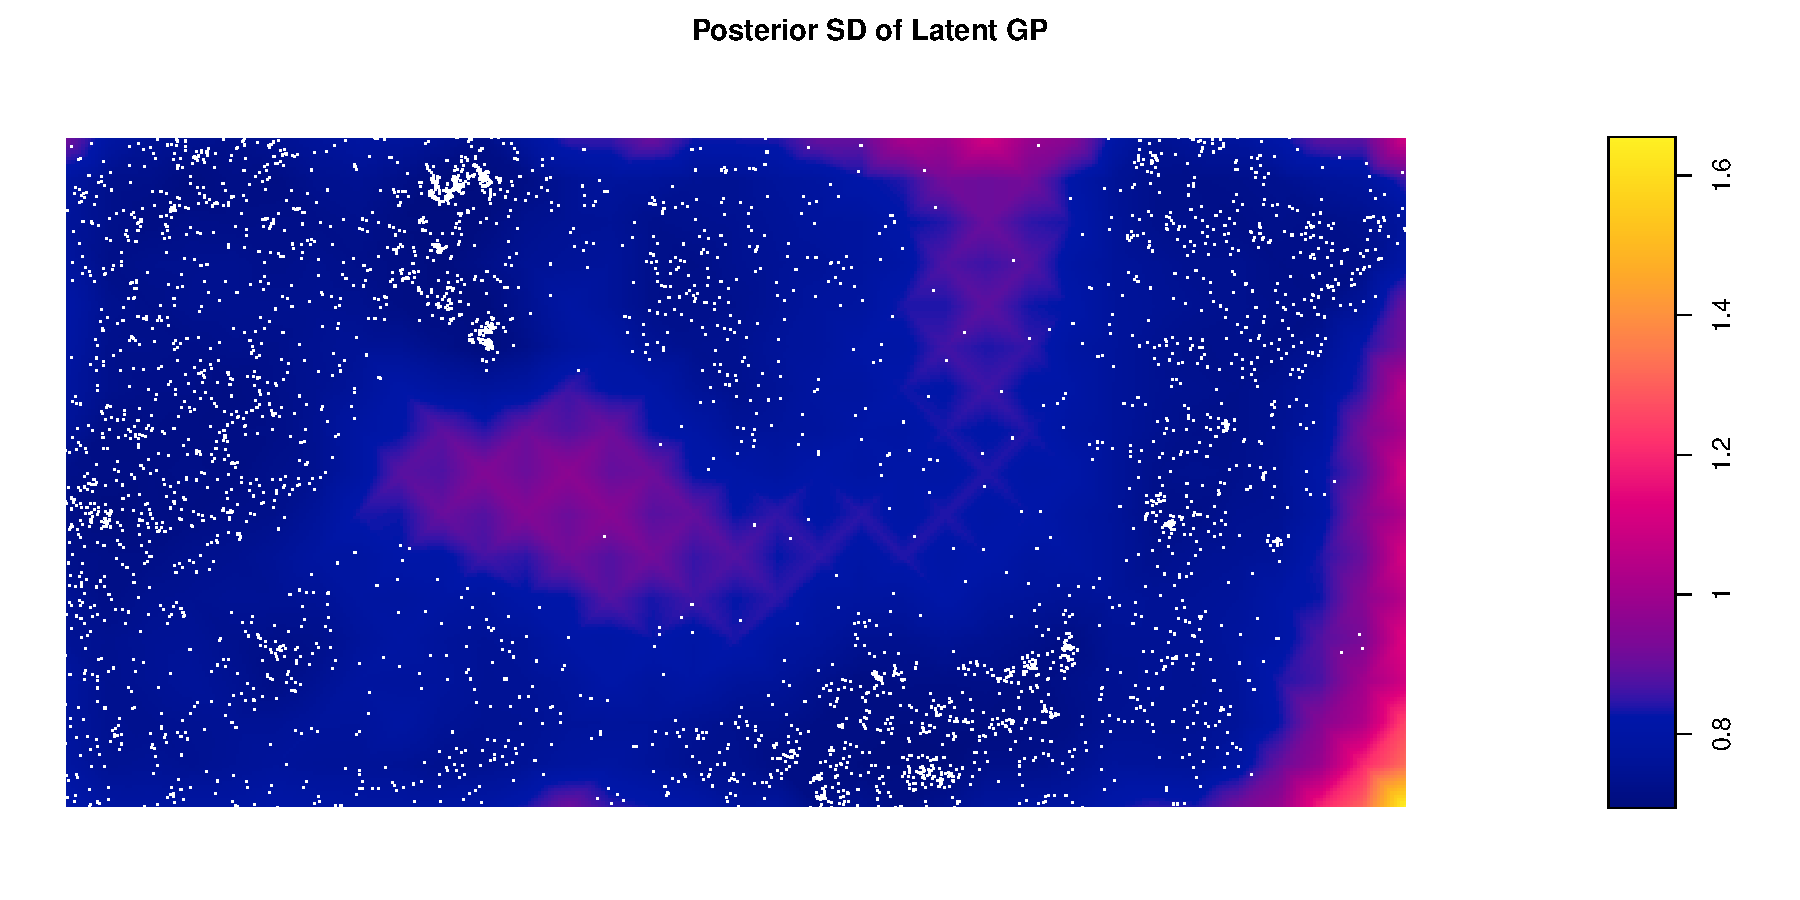
\includegraphics[width=\textwidth]{figures/beisd.pdf}
\caption{Pointwise posterior standard deviation of predictions.}
\label{beisd}
\end{figure}


\subsubsection{Results}


\subsubsection{Model Checking}


\section{Conclusion and Discussion}
%  {\bf Conclusion and Discussion:} In this conclusion and discussion section, provide conclusions of your review and provide anticipated future direction(s) in this area.


%\section*{Acknowledgement(s)}

%An unnumbered section, e.g.\ \verb"\section*{Acknowledgements}", may be used for thanks, etc.\ if required and included \emph{in the non-anonymous version} before any Notes or References.

%\section*{Disclosure statement}

%An unnumbered section, e.g.\ \verb"\section*{Disclosure statement}", may be used to declare any potential conflict of interest and included \emph{in the non-anonymous version} before any Notes or References, after any Acknowledgements and before any Funding information.

%\section*{Funding}

%An unnumbered section, e.g.\ \verb"\section*{Funding}", may be used for grant details, etc.\ if required and included \emph{in the non-anonymous version} before any Notes or References.

%\section*{Notes on contributor(s)}

%An unnumbered section, e.g.\ \verb"\section*{Notes on contributors}", may be included \emph{in the non-anonymous version} if required. A photograph may be added if requested.

%\section*{Nomenclature/Notation}

%An unnumbered section, e.g.\ \verb"\section*{Nomenclature}" (or \verb"\section*{Notation}"), may be included if required, before any Notes or References.

%\section*{Notes}

%An unnumbered `Notes' section may be included before the References (if using the \verb"endnotes" package, use the command \verb"\theendnotes" where the notes are to appear, instead of creating a \verb"\section*").

\bibliographystyle{tfs}
\bibliography{jas-inla-review}

\end{document}
